\chapter{Lab 3 Results: What Holds a GPT Together}\label{app:lab3}

This appendix presents the experimental results from Lab~3, which diagnoses the load-bearing components of a decoder-only Transformer. The method is \emph{build-up}: start from a minimal GPT, progressively add architectural features, and measure what each contributes to correctness, trainability, and inference efficiency.

\textbf{Task:} Character-level language modeling on Tiny Shakespeare. Model: 8-layer decoder-only Transformer, $d_\text{model}=128$, 4 heads. Training: 2000 steps, batch size 64, sequence length 256.

%----------------------------------------------------------------------
\section{Experiment 0: Shifted-Label Bug Hunt}

\textbf{Question:} What happens when the next-token prediction objective is incorrectly aligned?

\textbf{Setup:} Compare two loss functions on the same model:
\begin{itemize}
\item \textbf{Buggy:} \texttt{CE(logits.reshape(-1,V), input\_ids.reshape(-1))} --- predicts the current token, not the next one.
\item \textbf{Fixed:} \texttt{CE(logits[:,:-1].reshape(-1,V), input\_ids[:,1:].reshape(-1))} --- correctly shifted.
\end{itemize}

\textbf{Results:}

\begin{center}
\begin{tabular}{lccl}
\toprule
 & \textbf{Val Loss} & \textbf{Generation Quality} & \textbf{Failure Mode} \\
\midrule
Buggy (no shift) & 0.0077 & Repeated characters, garbage & Trivial copy \\
Fixed (shifted) & 2.39 & Beginning to resemble English & Genuine LM \\
\bottomrule
\end{tabular}
\end{center}

\begin{figure}[h]
\centering
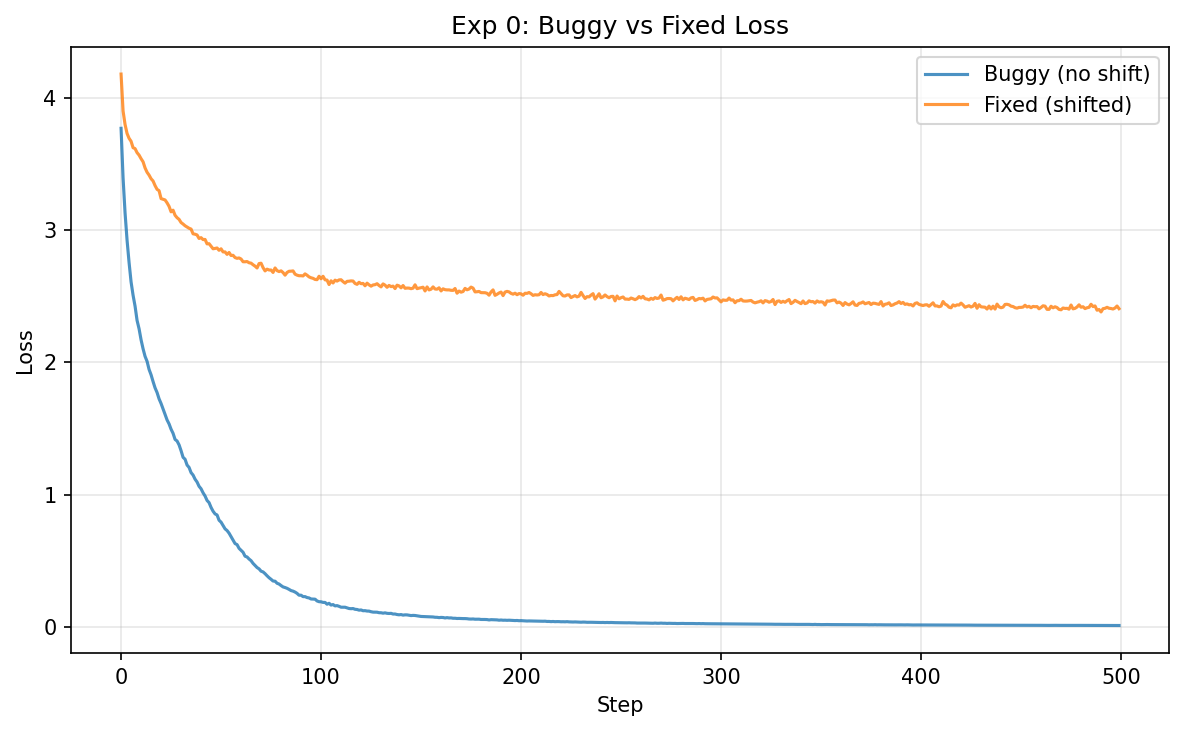
\includegraphics[width=0.65\textwidth]{labs/ch03/answers/figures/exp0_loss_comparison.png}
\caption{Training loss: buggy model converges to near-zero (trivial task); fixed model converges to a realistic loss level.}
\label{fig:app-lab3-exp0}
\end{figure}

\textbf{Diagnosis:} The buggy loss is trivially low because the model only needs to copy the current token from the input---no actual prediction required. This is the autoregressive equivalent of Lab~2's causal mask bug: \textbf{suspiciously low loss should trigger investigation, not celebration.} The shifted loss forces the model to predict the next token, which is the genuine language modeling objective.

\textbf{Core insight:} Labs 2 and 3 now form a pair of ``silent failure'' demonstrations:
\begin{itemize}
\item \textbf{Lab 2 Exp 1:} Remove causal mask $\to$ model copies from future targets $\to$ loss 0.003, accuracy 0\%.
\item \textbf{Lab 3 Exp 0:} Don't shift labels $\to$ model copies current token $\to$ loss 0.008, generation garbage.
\end{itemize}
Both produce \emph{near-zero loss with zero useful capability}. The mechanism differs (future leakage vs.\ target misalignment), but the diagnostic principle is identical: \textbf{loss measures how well the model solves the task you gave it, not the task you intended.} If you accidentally define a trivial task, the model will solve it trivially. The first checkpoint for any new model should always be: ``Does the generated output look reasonable?''---never rely on loss alone.

\textbf{Practical implication:} This bug is common in custom training loops. Library \texttt{CausalLM} classes often handle shifting internally, but hand-written losses often get it wrong. The rule is simple: if your loss sees logit at position $t$ and target at position $t$, you have this bug.

%----------------------------------------------------------------------
\section{Experiment 1: Residual Stream and Normalization (Centerpiece)}

\textbf{Question:} What makes an 8-layer decoder-only Transformer trainable?

\textbf{Setup:} Three configurations, all 8 layers:
\begin{enumerate}[label=(\Alph*)]
\item No residual connections, pre-norm
\item Residual connections, post-norm
\item Residual connections, pre-norm (baseline)
\end{enumerate}

\textbf{Results:}

\begin{center}
\begin{tabular}{lcccl}
\toprule
\textbf{Config} & \textbf{Val Loss} & \textbf{Gradient Behavior} & \textbf{Stable?} & \textbf{Generation} \\
\midrule
A: No residual & 3.35 & Unstable & Barely trains & Gibberish \\
B: Post-norm & 1.67 & Higher variance & Trains & Words, some errors \\
C: Pre-norm & 1.57 & Smooth & Best & Coherent phrases \\
\bottomrule
\end{tabular}
\end{center}

\begin{figure}[h]
\centering
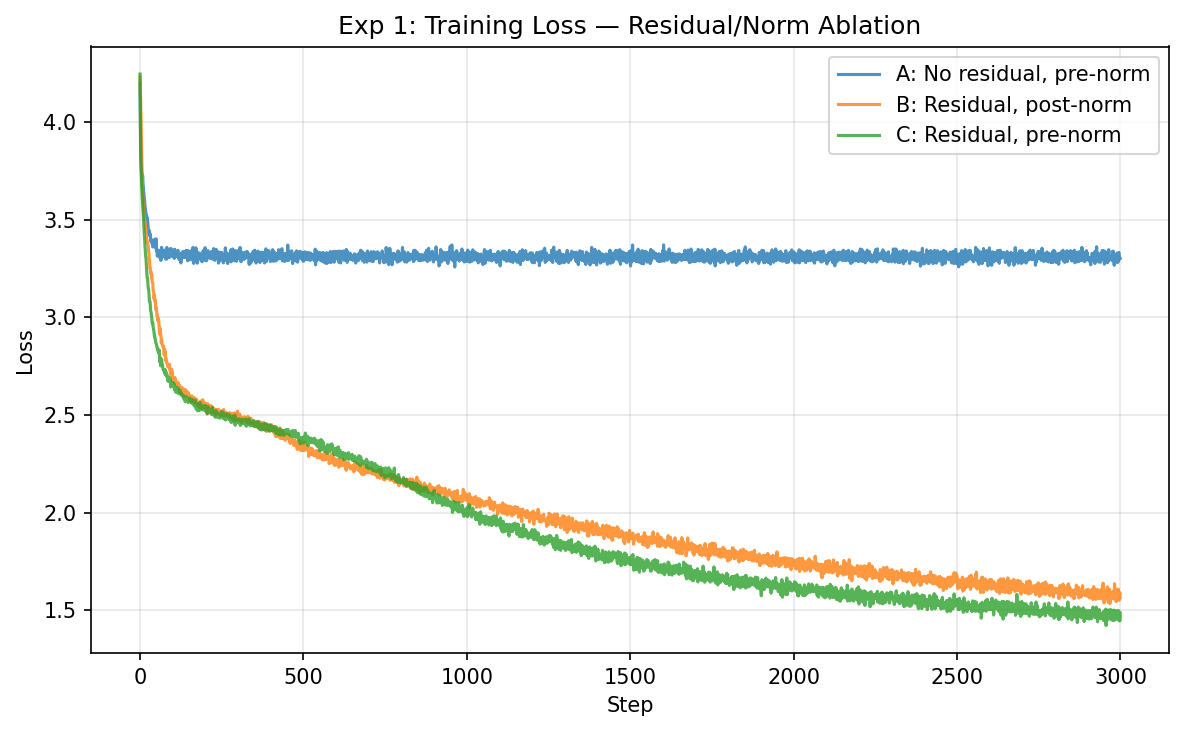
\includegraphics[width=0.7\textwidth]{labs/ch03/answers/figures/exp1_loss_comparison.png}
\caption{Training loss: no-residual model plateaus high; post-norm trains but lags; pre-norm converges fastest and lowest.}
\label{fig:app-lab3-exp1-loss}
\end{figure}

\begin{figure}[h]
\centering
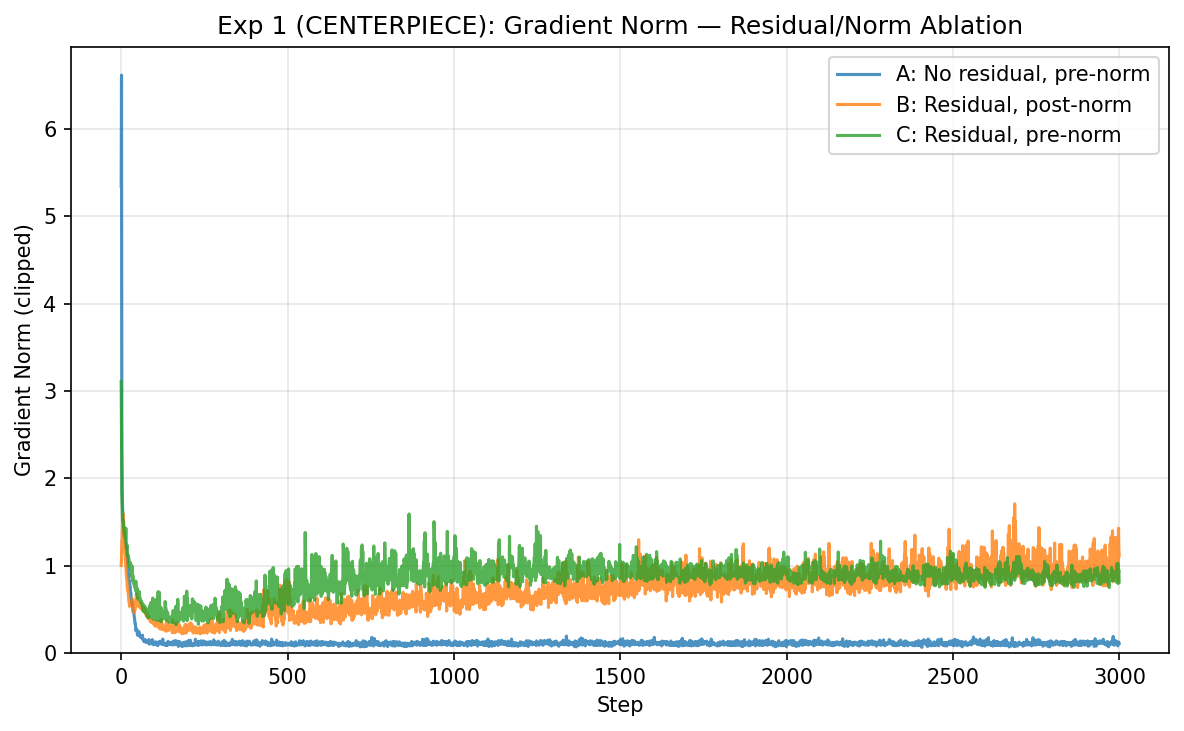
\includegraphics[width=0.7\textwidth]{labs/ch03/answers/figures/exp1_grad_norm_comparison.png}
\caption{Gradient norm comparison. No-residual model shows instability; pre-norm is smoothest.}
\label{fig:app-lab3-exp1-grad}
\end{figure}

\textbf{Diagnosis:} The residual stream is the gradient highway that makes deep Transformers trainable---closely analogous to the LSTM cell state highway from Lab~1. Without residual connections, gradients must pass through a deeper chain of transformations, producing the same kind of instability that vanilla RNNs exhibit. Pre-norm further stabilizes training by normalizing inputs to each sublayer, reducing scale drift across depth.

\textbf{Core insight:} This experiment answers Ch3's central question: \emph{what makes a decoder-only Transformer trainable?} Not attention---attention is the same in all three configurations. Not normalization alone---post-norm normalizes too. The answer is the \textbf{residual stream as an additive identity highway}: each layer computes $x + f(x)$ rather than $f(x)$. At initialization, $f(x) \approx 0$ (small random weights), so the residual stream passes inputs nearly unchanged. Gradients flow directly through the addition operator with gradient 1.0, regardless of depth. This is the same principle as LSTM's cell state ($c_t = f_t \odot c_{t-1} + i_t \odot \tilde{c}_t$): the additive path provides a gradient highway that multiplicative chains cannot.

The pre-norm vs.\ post-norm difference is subtler but important: pre-norm applies LayerNorm \emph{before} the sublayer, so the sublayer always receives normalized input. Post-norm applies it \emph{after}, which means the sublayer's output scale can drift---and at 8+ layers, this drift accumulates into training instability. This is why virtually all modern GPTs use pre-norm.

\textbf{Cross-Lab 1 parallel:}
\begin{center}
\begin{tabular}{lll}
\toprule
\textbf{Lab 1} & \textbf{Lab 3} & \textbf{Mechanism} \\
\midrule
Vanilla RNN fails at depth/distance & No-residual GPT fails at depth & No gradient highway \\
LSTM cell state $\to$ stable & Residual stream $\to$ stable & Additive bypass \\
RNN gradient norm: 60,241 & No-residual: unstable gradients & Multiplicative chain \\
LSTM gradient norm: 0.59 & Pre-norm: smooth gradients & Additive + normalized \\
\bottomrule
\end{tabular}
\end{center}

\textbf{Deeper implication:} The residual stream is not just a training trick---it shapes how the model represents information. In a residual network, each layer makes a \emph{small additive update} to a shared representation. This means the model can be understood as a ``stream of consciousness'' that is incrementally refined by successive attention and FFN operations. This perspective is the foundation of modern Transformer interpretability work (residual stream patching, activation patching, etc.).

%----------------------------------------------------------------------
\section{Experiment 2: Positional Encoding}

\textbf{Question:} How does position information enter a decoder-only model, and which encoding works best?

\textbf{Setup:} Three configurations:
\begin{enumerate}[label=(\Alph*)]
\item No positional encoding
\item Learned absolute PE
\item Rotary Position Embedding (RoPE)
\end{enumerate}

\textbf{Results:}

\begin{center}
\begin{tabular}{lccl}
\toprule
\textbf{Config} & \textbf{Val Loss} & \textbf{$\Delta$ vs RoPE} & \textbf{Generation Quality} \\
\midrule
A: No PE & 2.08 & +0.53 & Words exist but structure weak \\
B: Learned PE & 1.79 & +0.24 & Better sentence structure \\
C: RoPE & 1.55 & --- & Best coherence \\
\bottomrule
\end{tabular}
\end{center}

\begin{figure}[h]
\centering
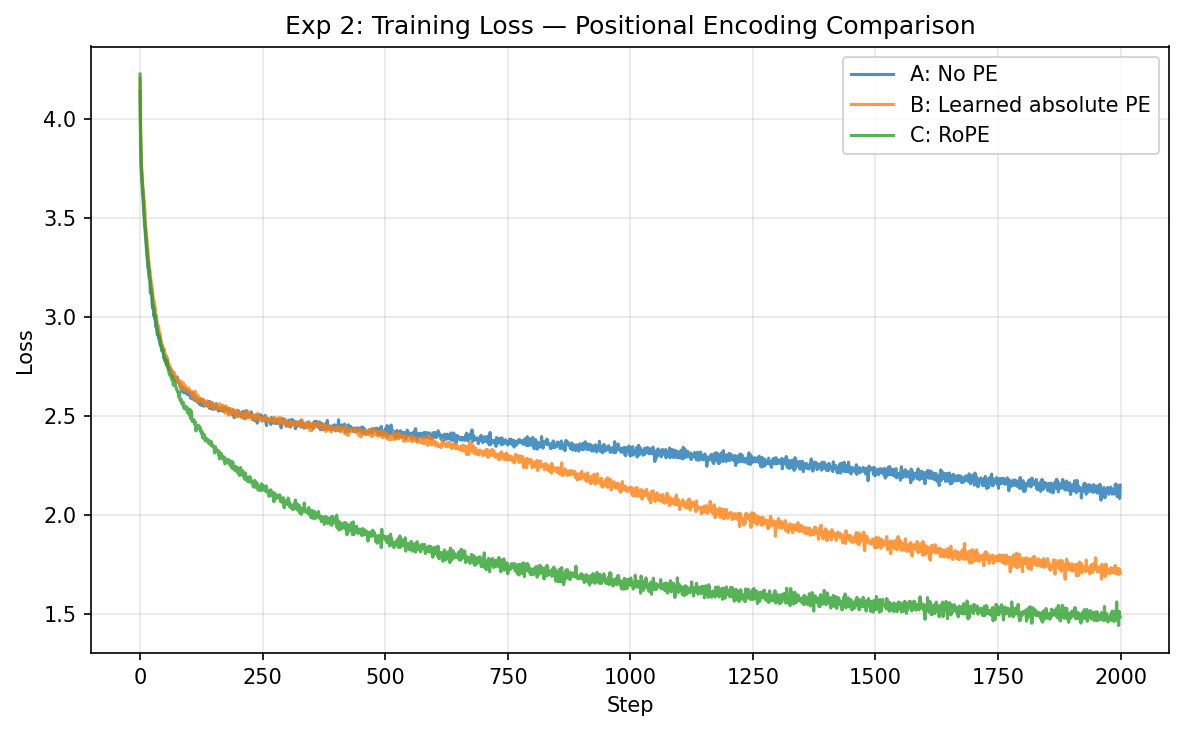
\includegraphics[width=0.65\textwidth]{labs/ch03/answers/figures/exp2_loss_comparison.png}
\caption{Training loss: no-PE model converges slower and to a higher loss; RoPE achieves the lowest loss.}
\label{fig:app-lab3-exp2}
\end{figure}

\textbf{Diagnosis:}
\begin{itemize}
\item \textbf{No PE does not fully collapse} because the causal mask still provides partial ordering (token at position 5 can see 5 tokens; token at position 100 can see 100). But the model cannot learn fine-grained positional patterns.
\item \textbf{Learned PE} gives each position a trainable vector. Works well within the trained context length.
\item \textbf{RoPE} encodes relative position through rotation of Q/K vectors, so the attention score between two tokens depends only on their distance. Even in a short training run (2000 steps), RoPE edges out learned PE.
\end{itemize}

\textbf{Core insight:} The no-PE result (val loss 2.08, not catastrophic) is itself informative. Why doesn't the model completely fail without positional information? Because the causal mask \emph{implicitly} provides ordering: the token at position 0 sees 1 token (itself), position 1 sees 2 tokens, position 100 sees 101 tokens. The model can learn ``I am early in the sequence'' vs.\ ``I am late'' from the number of visible tokens. But it cannot learn \emph{relative} structure: ``the word two positions ago was a verb'' requires knowing that the distance is exactly 2, not just ``I can see many tokens.''

This helps explain why RoPE outperforms learned absolute PE in this run: RoPE encodes \emph{relative} position directly in the Q$\cdot$K dot product. Two tokens that are 5 apart receive a consistent relative-position contribution regardless of their absolute positions. Learned absolute PE can \emph{implicitly} capture relative position through differences between learned vectors, but must learn this relationship from data---a harder task, especially in short training runs.

\textbf{Connection to Lab 2 Exp 3:} Lab~2 showed encoder PE is critical (97\% $\to$ 22\% without it) while decoder PE is less so (96.6\% without it). Lab~3 confirms the same pattern in a decoder-only setting: causal masking provides enough ordering for basic language modeling, but fine-grained positional awareness requires explicit PE. The threshold is: \emph{tasks that need exact positional reasoning} (reversal, morphological suffixing, counting) need PE most; tasks that can rely on coarse ordering (next-word prediction from long context) tolerate PE removal better.

%----------------------------------------------------------------------
\section{Experiment 3: KV Cache Profiling and Ablation}

\textbf{Question:} How does KV cache change autoregressive inference cost, and how does the advantage scale with model size and sequence length?

\subsection*{Baseline (tiny model)}

A tiny model ($d=128$, 8~layers, 1.6M params) generates 256 tokens: speedup = $1.06\times$. At this scale, KV cache barely matters. But is the mechanism correct? Yes---cached and uncached generation produce identical logits.

\subsection*{Ablation: model size $\times$ sequence length}

To understand \emph{when} KV cache matters, we ran five configurations varying both dimensions:

\begin{center}
\begin{tabular}{llcccc}
\toprule
\textbf{Config} & \textbf{Params} & \textbf{Gen Len} & \textbf{Slowdown} & \textbf{End Speedup} & \textbf{Peak Mem} \\
\midrule
A: tiny        & 1.6M  & 256  & $0.9\times$ & $0.8\times$ & 143 MB \\
B: medium      & 51M   & 512  & $1.1\times$ & $0.8\times$ & 1670 MB \\
C: medium+long & 51M   & 1024 & $\mathbf{2.6\times}$ & $\mathbf{2.5\times}$ & 1675 MB \\
D: large       & 85M   & 512  & $1.7\times$ & $1.8\times$ & 2273 MB \\
E: large+long  & 86M   & 1024 & $\mathbf{3.9\times}$ & $\mathbf{4.2\times}$ & 2279 MB \\
\bottomrule
\end{tabular}
\end{center}

``Slowdown'' = ratio of last-token to first-token time without cache (measures how much no-cache degrades with position).
``End speedup'' = no-cache last-token time $\div$ cache last-token time (KV cache advantage at end of generation).

\begin{figure}[h]
\centering
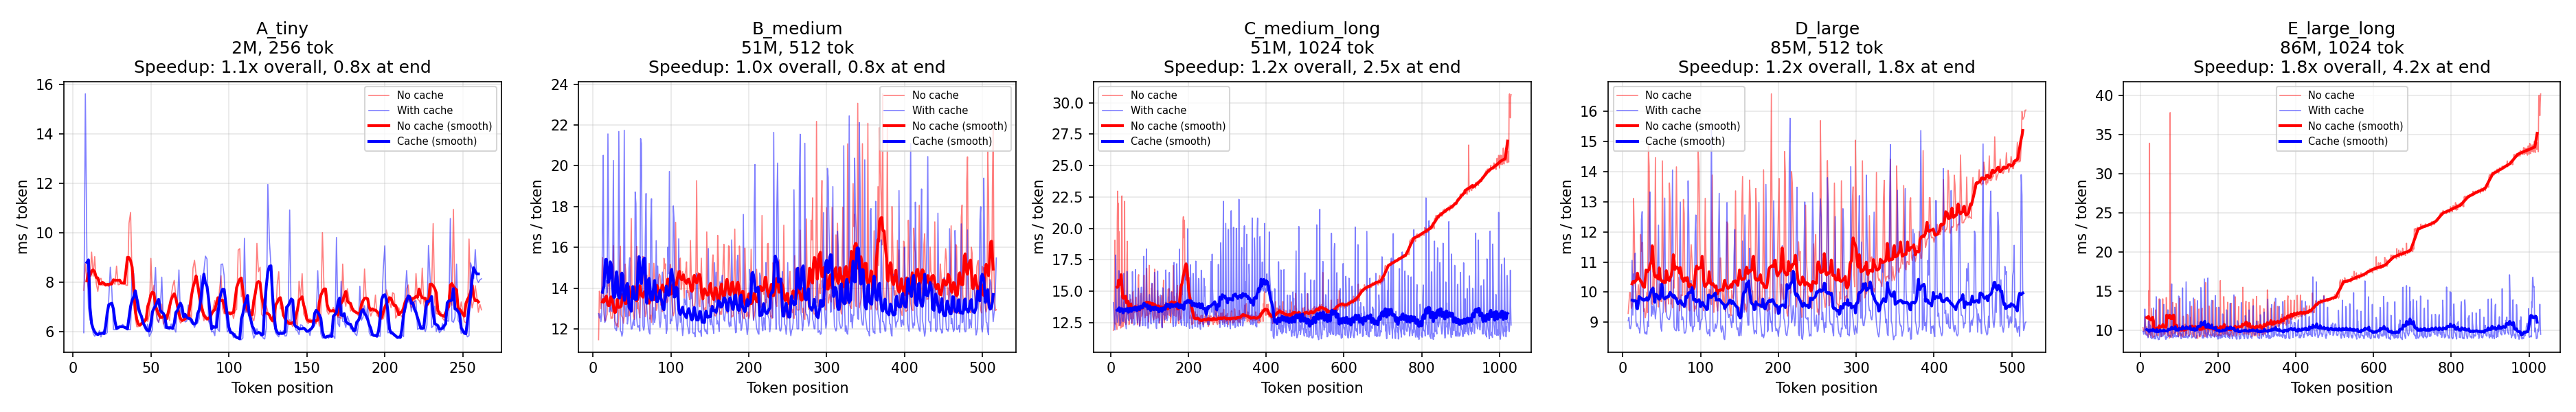
\includegraphics[width=\textwidth]{labs/ch03/answers/figures/exp3_kv_cache_ablation.png}
\caption{ms/token vs.\ generated position across five configurations. No-cache (red) grows with position; cache (blue) stays flat. The gap widens dramatically from A to E.}
\label{fig:app-lab3-exp3-ablation}
\end{figure}

\begin{figure}[h]
\centering
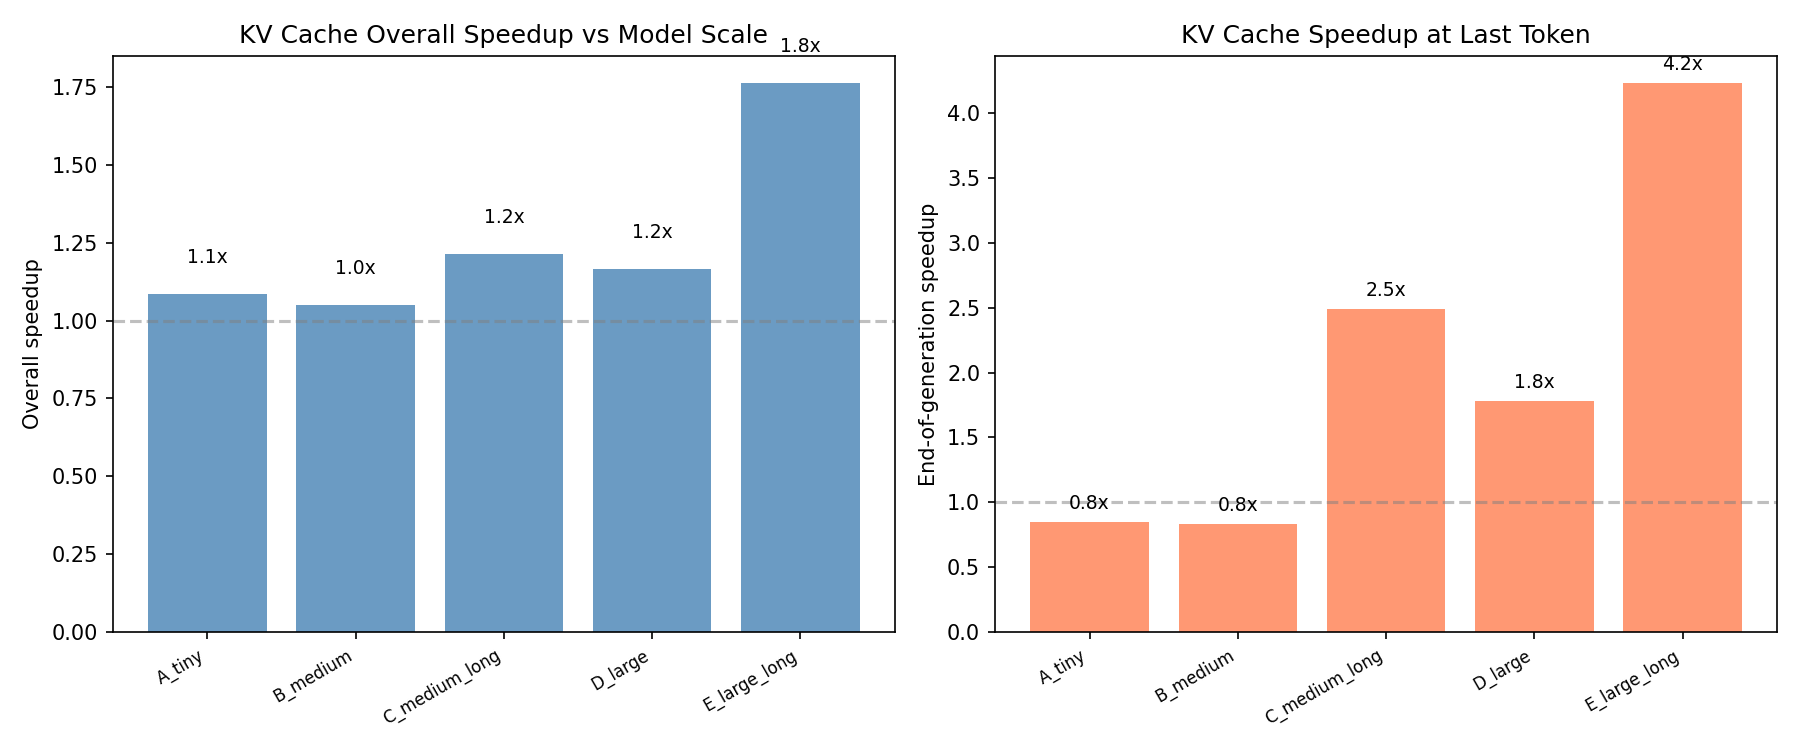
\includegraphics[width=0.7\textwidth]{labs/ch03/answers/figures/exp3_kv_cache_ablation_summary.png}
\caption{Overall speedup (left) and end-of-generation speedup (right) grow with both model size and sequence length.}
\label{fig:app-lab3-exp3-summary}
\end{figure}

\subsection*{Two-dimensional scaling analysis}

\textbf{Sequence length effect} (fixed model): B$\to$C (51M, 512$\to$1024 tokens) takes end speedup from $0.8\times$ to $\mathbf{2.5\times}$. D$\to$E (85M, 512$\to$1024) takes it from $1.8\times$ to $\mathbf{4.2\times}$. Doubling sequence length more than doubles the advantage.

\textbf{Model size effect} (fixed sequence): B$\to$D (512 tokens, 51M$\to$85M) takes end speedup from $0.8\times$ to $1.8\times$. C$\to$E (1024 tokens, 51M$\to$86M) takes it from $2.5\times$ to $4.2\times$. Larger models amplify the advantage because attention becomes a larger fraction of total compute.

\textbf{Core insight:} KV cache is not merely a small constant-factor tweak---it changes the decode-time cost structure. Instead of repeatedly recomputing the growing prefix, the model reuses previous K/V tensors and only computes the new token's query, key, and value. This distinction is invisible when $N$ is small (constant factors dominate), but becomes the difference between ``feasible'' and ``infeasible'' at production scale.

The ablation makes this concrete: the same mechanism that gives $0.8\times$ at (1.6M, 256 tokens) gives $4.2\times$ at (86M, 1024 tokens). Extrapolating to 7B-scale models at multi-thousand-token contexts, the speedup becomes large enough that KV cache is not an optional optimization but a \textbf{structural requirement} for practical deployment.

\textbf{Why the tiny model shows no advantage:} Three conditions must align---$T$ large enough for $O(T^2)$ attention to dominate over $O(d^2)$ FFN; $d$ large enough for matrix operations to be compute-bound rather than launch-bound; and sufficient depth for per-layer savings to accumulate. Config A violates all three. Config E satisfies all three. \textbf{The lesson:} when a toy experiment under-demonstrates a theoretical prediction, the discipline is to identify the regime conditions rather than dismissing the theory.

%----------------------------------------------------------------------
\section{Cross-Lab Comparison: LSTM vs Transformer}

\textbf{Question:} At matched parameter count, how do LSTM (Lab~1) and Transformer (Lab~3) compare on the same task?

\textbf{Setup:} Both trained on Tiny Shakespeare, 3000 steps, batch 64, seq\_len 256.
\begin{itemize}
\item LSTM: 2 layers, hidden=512, 3.3M parameters
\item Transformer: 4 layers, $d_\text{model}$=256, 4 heads, 3.2M parameters
\end{itemize}

\textbf{Results:}

\begin{center}
\begin{tabular}{lccc}
\toprule
 & \textbf{Val Loss} & \textbf{Tokens/sec} & \textbf{Speedup} \\
\midrule
LSTM & 1.469 & 360K & --- \\
Transformer & 1.499 & 783K & $2.2\times$ \\
\bottomrule
\end{tabular}
\end{center}

\begin{figure}[h]
\centering
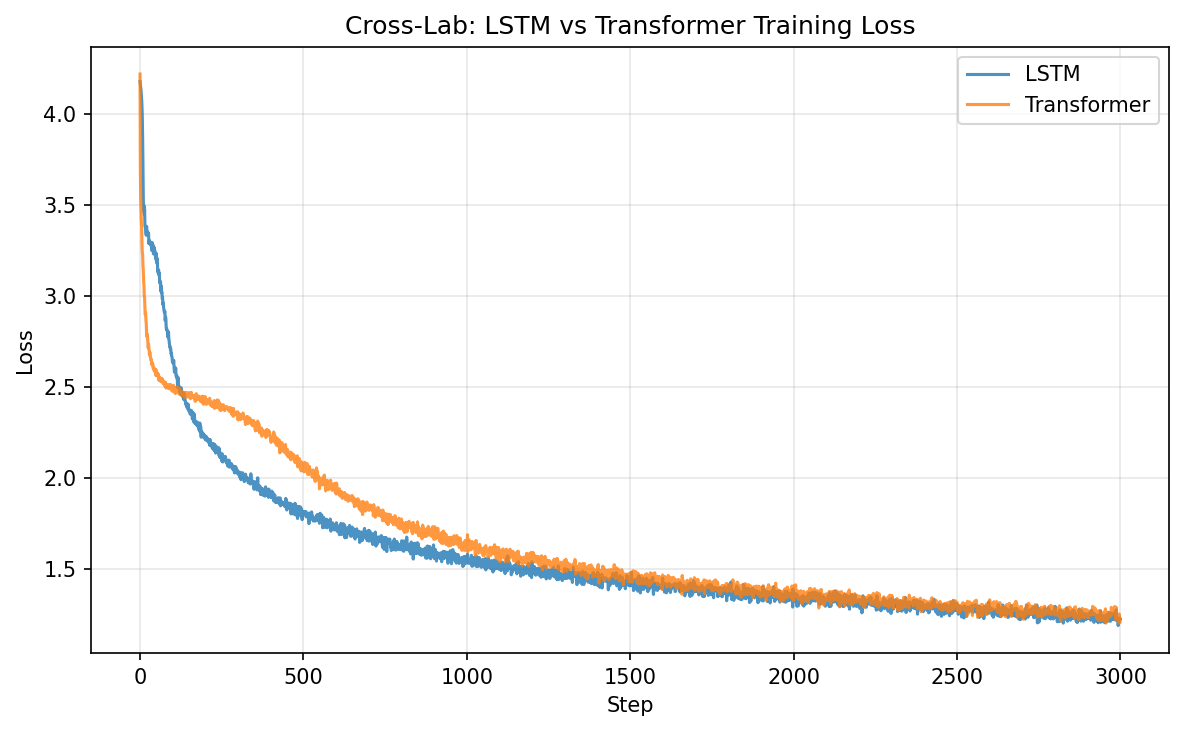
\includegraphics[width=0.65\textwidth]{labs/ch03/answers/figures/cross_lab_comparison.png}
\caption{LSTM vs.\ Transformer at $\sim$3M params. Loss is nearly identical; Transformer throughput is $2.2\times$ higher.}
\label{fig:app-lab3-crosslab}
\end{figure}

\textbf{Diagnosis:}
\begin{itemize}
\item At small scale and short training, LSTM and Transformer achieve nearly identical loss (difference: 0.03). The LSTM is even marginally better.
\item The Transformer's advantage at this scale is \textbf{training speed}: $2.2\times$ throughput due to full parallelism over the sequence dimension.
\item This result is pedagogically important: the Transformer did not win because it is ``smarter'' at 3M parameters. It wins because it is \textbf{faster to train}, which means it can be scaled to billions of parameters within practical compute budgets. The quality advantage emerges from scale---the subject of Part~II.
\end{itemize}

\textbf{Core insight:} This is perhaps the most important conceptual result in Lab~3. It directly challenges the naive narrative that ``Transformers are better than LSTMs because attention is more powerful than recurrence.'' At 3M parameters and 3000 steps, the LSTM \emph{matches or slightly beats} the Transformer on loss. So why did the field abandon LSTMs?

The answer begins with the $2.2\times$ throughput gap---and the source of this gap is architectural, not just an implementation accident. An LSTM must process token $t$ before token $t+1$ (serial dependency through hidden state). A Transformer processes all tokens in parallel during training. This means:
\begin{itemize}
\item With the same hardware and time budget, you can train a Transformer on $2.2\times$ more tokens.
\item Alternatively, you can train a $2.2\times$ larger Transformer in the same time.
\item Compound over thousands of GPU-hours, this advantage is multiplicative with scale.
\end{itemize}

\textbf{The implication:} Transformers won not because they always model language better at fixed small scale, but because they \emph{scale better}. At 3M params in this experiment, LSTM $\approx$ Transformer. At billion-parameter scale, decoder-only Transformers become far more useful in practice---not because attention magically dominates recurrence at every size, but because parallelism makes it feasible to train much larger models on much more data. \textbf{Architecture enables scale; scale produces capability.} This is the thesis of Part~II.

\textbf{A nuance:} The LSTM's serial bottleneck also makes it harder to utilize modern GPUs (which are optimized for parallel matrix operations). The 360K vs.\ 783K tokens/sec gap can widen on larger accelerators, because recurrence exposes less sequence-level parallelism while the Transformer can batch the full context during training.

%----------------------------------------------------------------------
\section{Synthesis}

\begin{center}
\begin{tabular}{llll}
\toprule
\textbf{Property} & \textbf{Load-Bearing Component} & \textbf{Without It} & \textbf{Evidence} \\
\midrule
Correctness & Shifted labels + causal mask & Fake-low loss, broken gen & Exp 0 \\
Trainability & Residual stream + pre-norm & Gradient collapse at depth & Exp 1 \\
Word order & Positional encoding & Structure degradation & Exp 2 \\
Inference speed & KV cache & $O(T^2)$ per step & Exp 3 \\
Scale advantage & Parallelism & No throughput gain & Cross-lab \\
\bottomrule
\end{tabular}
\end{center}

The decoder-only Transformer is not simply ``attention stacked many times.'' It is a system where each component addresses a specific failure mode. Remove any one, and a measurable degradation appears.

\subsection{The Three-Lab Arc}

Stepping back across all three labs, the course's experimental evidence forms a single argument:

\begin{enumerate}
\item \textbf{Lab 1:} Fixed representations fail (polysemy collapse). Sequential processing fails at distance (gradient pathology, memory decay). Gates add structure that fixes both---but serial processing remains. Attention removes the Seq2Seq bottleneck---but the model is still recurrent.

\item \textbf{Lab 2:} Attention alone is insufficient (rank collapse, saturation). The full Transformer block---residual + FFN + mask + PE + scaling---is a \emph{system}, not a single mechanism. Each ingredient addresses a specific failure mode.

\item \textbf{Lab 3:} Assembling these blocks into a decoder-only GPT requires additional engineering: correct objective alignment (shifted labels), depth-enabling structure (residual stream + pre-norm), positional awareness (RoPE), and inference optimization (KV cache). The resulting model matches LSTM quality at small scale but trains $2.2\times$ faster---a throughput advantage that compounds into the scaling revolution of Part~II.
\end{enumerate}

\textbf{The unifying principle across all three labs:} \emph{The simplest version of each idea does not work. What makes it work is careful engineering around the core mechanism's failure modes.} N-grams need smoothing. RNNs need gates. Attention needs residuals and normalization. GPTs need shifted labels and positional encoding. At every level of abstraction, the story is the same: identify the failure mode, add the minimal structure that fixes it, verify experimentally that the fix works and the failure mode is gone.
